\documentclass[11pt]{article}
\usepackage[letterpaper,margin=1in]{geometry}
\usepackage[T1]{fontenc}
\usepackage{amsmath,amsthm}
\usepackage{newtxtext,newtxmath}
\usepackage{microtype,graphicx,booktabs,array}
\usepackage[numbers,sort&compress]{natbib}
\usepackage{enumitem,placeins}
\usepackage{xcolor}
\definecolor{linkblue}{RGB}{24,69,102}
\usepackage[colorlinks=true,allcolors=linkblue]{hyperref}
\usepackage[nameinlink,noabbrev]{cleveref}
\crefname{proposition}{proposition}{propositions}
\crefname{corollary}{corollary}{corollaries}
\crefname{assumption}{assumption}{assumptions}
\hypersetup{pdftitle={Thermally driven nonlocal heat flux with electron-ion collisions}}
\widowpenalty=10000
\clubpenalty=10000
\setlist{nosep,leftmargin=*}
\setlength{\emergencystretch}{2em}
\setlength{\parskip}{3pt}
\newcommand{\dd}{\,\mathrm d}
\newcommand{\av}[1]{\left\langle #1\right\rangle}
\newcommand{\D}{\mathcal D}
\newcommand{\A}{\mathcal A}
\newcommand{\N}{\mathcal N}
\newcommand{\Q}{\mathcal Q}
\renewcommand{\P}{\mathcal P}
\newcommand{\kap}{\kappa}
\newcommand{\RR}{\mathbb R}
\newcommand{\dual}[1]{\left\langle #1,\Lambda^+ #1\right\rangle}
\newcommand{\thr}{\mathrm{th}}
\newcommand{\pot}{\mathrm{pot}}
\newtheorem{theorem}{Theorem}[section]
\newtheorem{proposition}[theorem]{Proposition}
\newtheorem{corollary}[theorem]{Corollary}
\theoremstyle{definition}
\newtheorem{assumption}[theorem]{Assumption}
\theoremstyle{remark}
\newtheorem{remark}[theorem]{Remark}
\numberwithin{equation}{section}
\title{\bfseries Thermally driven nonlocal heat flux\\ with electron--ion collisions:\\
extending the variational closure bounds}
\author{}
\date{17 November 2026}
\begin{document}
\maketitle
\vspace{-1.5em}
\begin{abstract}
The companion manuscript on nonlocal heat-flux closure studies a
potential-driven response for like-particle collision operators. Two of
its limitations matter for applications. In three velocity dimensions the
response has a stress cross term, so positivity and the Fourier upper
bound are only proved at small wavenumber. And the collision models
conserve momentum, so they do not describe electrons scattering on ions.
In this note we remove both limitations. We replace the potential drive
by an isotropic heating source. The temperature response is then a
diagonal entry of the kinetic resolvent, and the one-dimensional dual
variational principle carries over to three dimensions. For every
symmetric, nonnegative collision operator whose kernel contains the
density and energy invariants, we obtain
$\kap/(1+Kk^2)\leq\chi_\thr(k)\leq\kap$ at every wavenumber, where $\kap$
is the conductivity at zero current and $K$ is the sharp leading
coefficient. The hypotheses do not include momentum conservation, so the
result covers electron--electron Landau collisions together with
pitch-angle scattering on ions of charge $Z$. We derive the exact
thermally driven Dougherty response, which has
$K=16/(45\nu^2)$ and a collisionless coefficient $\tfrac95\sqrt{2/\pi}$,
both different from the potential-driven values. Galerkin calculations
reproduce Braginskii's electron coefficients at low degree and approach
the Spitzer--H\"arm and Lorentz-limit values as the degree and $Z$
increase. The normalized deficit coefficient $K/\kap^2$ grows roughly
linearly in $Z$, from about $4.3$ at $Z=1$ to $96$ at $Z=64$. In an
embedded test, the decay of a temperature perturbation in the
quasi-neutral kinetic model is reproduced by the quasi-static closure to
within $2\%$ for $Z=1$ at $|k|\lambda_e\leq0.3$, where
Spitzer--H\"arm conduction is off by $42\%$.
\end{abstract}

\section{Introduction}

The manuscript \emph{Nonlocal heat-flux closure across collision models}
(the ``companion manuscript'' below) defines a heat-flux closure as the
slow-frequency response of a linearized kinetic equation to a potential
force. It proves two-sided bounds for that response and computes it for
BGK, Dougherty and like-particle Landau collisions. We would like to use
those results as tests for electron heat-flux closures, which is where
nonlocal transport matters most in practice. Two things stand in the way.

The first is the drive. In three velocity dimensions the potential-driven
temperature response is an off-diagonal entry of the resolvent. The
companion manuscript shows that the resulting stress cross term prevents
an all-wavenumber proof of positivity or of $\chi\leq\kap$, and for Landau
collisions both questions are left open. Moreover, a potential force is
not how electron temperature perturbations are produced. Electrons are
heated, and the ambipolar electric field then adjusts so that no current
flows.

The second is the collision operator. Electrons collide with ions as well
as with each other. Electron--ion scattering does not conserve electron
momentum, and its rate grows like $|v|^{-3}$ at low speed and is
proportional to the ion charge $Z$. The local limit is then the
Spitzer--H\"arm conductivity \cite{SpitzerHarm1953,Braginskii1965}, which
involves a thermoelectric correction and has no analogue in the
momentum-conserving models.

In this note we address both. Our results are as follows.
\begin{itemize}
\item \emph{A thermal drive makes the three-dimensional problem as clean
as the one-dimensional one.} If the kinetic equation is driven by an
isotropic heating source, the heat flux is exactly $1/(ik)$ per unit
heating, the current vanishes, and the temperature response is a positive
quadratic form (\cref{thm:dual}). We obtain all-wavenumber bounds
(\cref{cor:bounds}) and the sharp leading coefficient with an $O(k^4)$
remainder (\cref{thm:leading}). For like-particle Landau collisions this
gives the positivity and the Fourier upper bound that are open for the
potential drive, under the same form-domain hypotheses.
\item \emph{The drive matters.} Both responses are entries of one
positive-definite $2\times2$ matrix of parallel and perpendicular
temperature responses (\cref{prop:matrix}). They share the conductivity
but not the leading deficit: for Dougherty the two coefficients are
$2/15$ and $16/45$, and for Landau $22.35$ and $26.36$.
\item \emph{Momentum conservation is not needed.} The theorems hold for
electron--electron plus electron--ion collisions with $\kap$ replaced by
the zero-current conductivity. We compute $\kap$, $K$ and the response
curves for $Z$ from $1$ to $64$ (\cref{sec:numerics}).
\item \emph{The closure works as an evolution law in this setting.}
Quasi-neutrality removes the fast dynamics that caused the transient
errors in the companion manuscript, and the quasi-static closure tracks
the kinetic decay of a temperature perturbation closely
(\cref{sec:embedded}).
\end{itemize}

We are careful about what we do not do. Everything is linear, about a
homogeneous Maxwellian, with one spatial Fourier direction, no magnetic
field and immobile ions. The theorems assume that the stationary problems
are solvable in the form domain, as in the companion manuscript; we do
not prove a weighted existence theorem for the electron operator. The
numerical values are Galerkin approximations with refinement diagnostics
and no certified error bars.

\section{The thermally driven response}\label{sec:thermal}

\subsection{Setting}

We use the notation and units of the companion manuscript in three
velocity dimensions: $M(v)=(2\pi)^{-3/2}e^{-|v|^2/2}$,
$\av b=\int bM\dd v$, and
\[
 n=\av h,\quad u=\av{v_xh},\quad T=\av{\zeta h},\quad q=\av{Qh},\qquad
 \zeta=\frac{|v|^2-3}{3},\quad Q=\frac12v_x(|v|^2-5).
\]
The collision operator $\Lambda$ is real, symmetric and nonnegative in
$L^2(M)$ and commutes with reflection in $v_x$. We write
$\D(f,h)=\av{f\Lambda h}$, $\D[f]=\D(f,f)$, and
$\dual b=\sup_f\{2\av{bf}-\D[f]\}$ for $b$ orthogonal to the kernel $\N$
of $\Lambda$. Within the axisymmetric class we assume only
\begin{equation}
 \operatorname{span}\{1,|v|^2\}\subseteq\N\subseteq
 \operatorname{span}\{1,v_x,|v|^2\}.
 \label{eq:kernel}
\end{equation}
The right-hand inclusion is an equality for like-particle operators. For
electrons scattering on immobile ions, the left-hand one is.

Instead of a force, we drive the kinetic equation with a heating source
that is isotropic in velocity:
\begin{equation}
 \partial_th+v_x\partial_xh+\Lambda h=p(t,x)\,\zeta(v)+a(t,x)\,v_x .
 \label{eq:kinetic}
\end{equation}
Since $\av\zeta=\av{v_x\zeta}=0$ and $\tfrac32\av{\zeta^2}=1$, the source
adds energy at the rate $p$ and adds no particles or momentum. The force
$a$ is at our disposal. Because $\Lambda1=0$, a force changes a stationary
solution only by the constant $a/(ik)$, which has zero temperature and
heat flux. In an electron plasma this is the ambipolar field, and we can
use it to set the density perturbation to zero.

For a spatial mode $e^{ikx}$ with $k\ne0$, let $\A_k=ikv_x+\Lambda$ and let
\begin{equation}
 g=\A_k^{-1}\zeta=g_e+iw
 \label{eq:g}
\end{equation}
be the stationary solution for unit heating, with $g_e$ real and even in
$v_x$ and $w$ real and odd. Unlike the potential-driven problem, there is
no ordered limit here: a spatially periodic heating source with zero mean
has a genuine steady state.

\begin{assumption}[Form solvability]\label[assumption]{ass:form}
The stationary solution \eqref{eq:g} exists, the moments and pairings
displayed below are finite, and the parity components $g_e$, $w$ are
admissible test functions for the forms $\Q_k$ and $\P_k$ defined in
\eqref{eq:forms}.
\end{assumption}

\subsection{Dual certificates at every wavenumber}

For an even trial $\varphi$ and an odd trial $\psi$ define
\begin{align}
 \Q_k[\varphi]&=\D[\varphi]+k^2\dual{v_x\varphi},
   &v_x\varphi&\perp\N,\nonumber\\
 \P_k[\psi]&=\D[\psi]+\dual{\zeta+kv_x\psi},
   &\zeta+kv_x\psi&\perp\N.
 \label{eq:forms}
\end{align}
The first constraint is $\av{v_x^2\varphi}=0$ when momentum is conserved
and is empty otherwise. The second is
$\av{v_x\psi}=0$ and $k\av{v_x|v|^2\psi}=-2$.

\begin{theorem}[Thermal response]\label{thm:dual}
Under \eqref{eq:kernel} and \cref{ass:form}, the stationary solution
\eqref{eq:g} satisfies
\begin{equation}
 \av{v_xg}=0,\qquad \av{Qg}=\frac1{ik},\qquad
 T_1:=\av{\zeta g}=\D[g_e]+\D[w]>0 .
 \label{eq:identities}
\end{equation}
Consequently the conductivity
\begin{equation}
 \chi_\thr(k):=-\frac{\av{Qg}}{ik\,T_1}=\frac1{k^2T_1}
 \label{eq:chith}
\end{equation}
is positive at every nonzero wavenumber. Moreover, for all admissible
trials,
\begin{equation}
 \frac{\av{\zeta\varphi}^2}{\Q_k[\varphi]}\leq T_1\leq\P_k[\psi],
 \label{eq:certificates}
\end{equation}
with equality at $\varphi=g_e$ and $\psi=w$.
\end{theorem}

\begin{proof}
The mean of $\A_kg=\zeta$ is $ik\av{v_xg}=\av\zeta=0$. Pairing with
$(|v|^2-3)/2$, which is a collision invariant, and using
$\tfrac12v_x(|v|^2-3)=Q+v_x$ gives $ik\av{(Q+v_x)g}=\tfrac32\av{\zeta^2}=1$.
These are the first two identities. The real and imaginary parts of
$\A_kg=\zeta$ are
\begin{equation}
 \Lambda g_e-kv_xw=\zeta,\qquad \Lambda w+kv_xg_e=0 .
 \label{eq:parity}
\end{equation}
Pairing the first with $g_e$ and the second with $w$, and adding, gives
$T_1=\av{\zeta g_e}=\D[g_e]+\D[w]\geq0$. If $T_1=0$, then $g_e,w\in\N$,
so $w=cv_x$ and the first equation reads $-kcv_x^2=\zeta$, which is
impossible. Hence $T_1>0$.

For admissible trials let $b=\zeta+kv_x\psi$. Then
\[
 |\av{\zeta\varphi}|\leq|\av{b\varphi}|+|k\av{v_x\varphi\,\psi}|
 \leq\dual b^{1/2}\D[\varphi]^{1/2}
      +|k|\dual{v_x\varphi}^{1/2}\D[\psi]^{1/2},
\]
and Cauchy--Schwarz in $\RR^2$ gives
$\av{\zeta\varphi}^2\leq\Q_k[\varphi]\,\P_k[\psi]$. Finally,
\eqref{eq:parity} shows that $g_e$ and $w$ are admissible, since
$kv_xg_e=-\Lambda w$ and $\zeta+kv_xw=\Lambda g_e$ are orthogonal to $\N$,
and that $\Q_k[g_e]=\P_k[w]=\D[g_e]+\D[w]=T_1$. Taking one trial at its
optimum proves \eqref{eq:certificates}.
\end{proof}

The proof is the one-dimensional proof of the companion manuscript. What
changed is the source. With a potential drive the source is $1$ and the
temperature is read off against $\zeta$, an off-diagonal pairing. With a
thermal drive the source and the observable are the same function, and
positivity is automatic.

\subsection{Bounds and the leading coefficient}

We now make the bounds explicit. If $v_x\in\N$ set $\lambda=0$. Otherwise
set $\lambda=L_{12}/L_{11}$, where
$L_{11}=\dual{v_x}$ and $L_{12}=\av{v_x,\Lambda^+Q}$. Define
\begin{equation}
 J=Q-\lambda v_x,\qquad \Lambda\Xi=J,\quad\Xi\perp\N,\qquad
 \kap=\av{J\Xi},\qquad
 b_*=\zeta-\frac{v_x\Xi}{\kap},\qquad C=\dual{b_*},\quad K=\kap C .
 \label{eq:constants}
\end{equation}
In both cases $\av{v_x\Xi}=0$, either by the choice of $\Xi$ or by the
choice of $\lambda$, so $\kap=\av{Q\Xi}$. When momentum is conserved,
$\kap=\av{Q,\Lambda^+Q}$ is the conductivity $\kappa_{\mathrm F}$ of the
companion manuscript. Otherwise, with $L_{22}=\dual Q$,
\begin{equation}
 \kap=L_{22}-\frac{L_{12}^2}{L_{11}}
 \label{eq:schur}
\end{equation}
is the heat conductivity at zero current: $L_{11}$ is the electrical
conductivity, $L_{12}$ the thermoelectric coefficient, and $\kap$ the
Schur complement. The source $b_*$ is orthogonal to $\N$, because
$\av{v_x\Xi}=0$ and $\av{v_x|v|^2\Xi}=2\av{Q\Xi}+5\av{v_x\Xi}=2\kap$.

\begin{corollary}[All-wavenumber bounds]\label[corollary]{cor:bounds}
If the quantities in \eqref{eq:constants} are finite, then for every
$k\ne0$
\begin{equation}
 \frac{\kap}{1+Kk^2}\leq\chi_\thr(k)\leq\kap .
 \label{eq:bounds}
\end{equation}
\end{corollary}

\begin{proof}
Take $\varphi_0=\tfrac12(|v|^2-5)-\lambda$. It lies in $\N$, so
$\D[\varphi_0]=0$; it satisfies $v_x\varphi_0=J\perp\N$ and
$\av{\zeta\varphi_0}=1$. Hence $\Q_k[\varphi_0]=k^2\kap$ and
$T_1\geq1/(k^2\kap)$. Next take $\psi_*=-\Xi/(k\kap)$. Then
$\zeta+kv_x\psi_*=b_*$ and $\D[\psi_*]=\av{J\Xi}/(k\kap)^2=1/(k^2\kap)$, so
$T_1\leq1/(k^2\kap)+C$. Insert both in \eqref{eq:chith}.
\end{proof}

\begin{assumption}[Second-order solve]\label[assumption]{ass:second}
Let $\Lambda G=b_*$. Choose $n_0\in\operatorname{span}\{1,|v|^2\}$ so that
$\widetilde G=G+n_0$ satisfies $\av{\zeta\widetilde G}=0$ and
$v_x\widetilde G\perp\N$, and assume $B=\dual{v_x\widetilde G}<\infty$.
\end{assumption}

\begin{theorem}[Leading coefficient]\label{thm:leading}
Under the hypotheses above and \cref{ass:second}, as $k\to0$,
\begin{equation}
 1-\frac{\chi_\thr(k)}{\kap}=Kk^2+O(k^4).
 \label{eq:leading}
\end{equation}
\end{theorem}

\begin{proof}
Let $\Q_k(\cdot,\cdot)$ be the bilinear form of $\Q_k$. The stationary
equations give $\Q_k(g_e,\varphi)=\av{\zeta\varphi}$, and hence
$\Q_k[g_e-\varphi]=T_1-(2\av{\zeta\varphi}-\Q_k[\varphi])$. Put
$\varepsilon=k^2\kap$ and $\varphi'=\varphi_0+\varepsilon\widetilde G$, so
$\av{\zeta\varphi'}=1$. Using $\Lambda^+(v_x\varphi_0)=\Xi$ and
$v_x\Xi=\kap(\zeta-b_*)$,
\[
 \Q_k[\varphi']=\varepsilon^2C+k^2\bigl(\kap
   +2\varepsilon\kap\av{(\zeta-b_*)\widetilde G}+\varepsilon^2B\bigr)
   =\varepsilon\bigl(1-\varepsilon C+\varepsilon k^2B\bigr).
\]
Taking $\varphi=\varphi'/\Q_k[\varphi']$ gives
$T_1\geq1/\Q_k[\varphi']\geq\varepsilon^{-1}+C-Bk^2$ for small $k$, and
\cref{cor:bounds} gives $T_1\leq\varepsilon^{-1}+C$. Therefore
$\chi_\thr/\kap=1/(\varepsilon T_1)=1-\kap Ck^2+O(k^4)$.
\end{proof}

Three remarks are in order. First, the global constant in
\eqref{eq:bounds} is sharp at the origin, exactly as in one dimension.
Second, the remainder is $O(k^4)$, where the potential-driven result in
three dimensions only gives $O(|k|^3)$; the stress response no longer
enters. Third, for like-particle Landau collisions the constants in
\eqref{eq:constants} and \cref{ass:second} involve collision inverses of
polynomial sources orthogonal to the invariants, which exist in the
weighted energy class by the proposition on weighted solvability in the
companion manuscript. The stationary solution \eqref{eq:g} is a
resolvent applied to $\zeta$ rather than to $1$, and we have not written
out that case; it is covered by \cref{ass:form}.

\section{Why the drive matters}\label{sec:matrix}

Let $a_\parallel=v_x^2-1$ and $a_\perp=v_\perp^2/2-1$, so that
$\zeta=(a_\parallel+2a_\perp)/3$, and let
\begin{equation}
 M_{ij}(k)=\av{a_i,\A_k^{-1}a_j},\qquad i,j\in\{\parallel,\perp\}.
 \label{eq:matrix}
\end{equation}
This is the response of the parallel and perpendicular temperatures to
parallel and perpendicular heating.

\begin{proposition}[One matrix, two closures]\label[proposition]{prop:matrix}
Under the analogue of \cref{ass:form} for the sources $a_\parallel$ and
$a_\perp$, the matrix $M(k)$ is real, symmetric and positive definite, and
\begin{equation}
 \chi_\thr=\frac{9}{k^2\,(M_{\parallel\parallel}+4M_{\parallel\perp}
     +4M_{\perp\perp})} .
 \label{eq:chithM}
\end{equation}
If, in addition, $\Lambda$ conserves momentum, then the potential-driven
conductivity of the companion manuscript is
\begin{equation}
 \chi_\pot=\frac{3}{k^2\,(M_{\parallel\parallel}+2M_{\parallel\perp})} .
 \label{eq:chipotM}
\end{equation}
\end{proposition}

\begin{proof}
For real $c\in\RR^2$ and $a_c=c_\parallel a_\parallel+c_\perp a_\perp$,
the argument of \cref{thm:dual} gives
$\av{a_c,\A_k^{-1}a_c}=\D[g_e]+\D[w]>0$ for the corresponding solution.
Symmetry follows from the bilinear symmetry of $\A_k$, and the entries
are real because the sources are even. Equation \eqref{eq:chithM} is
\eqref{eq:chith} with $\zeta=(a_\parallel+2a_\perp)/3$. If
$\Lambda v_x=0$, then $\A_kv_x=ikv_x^2$, so
$\A_k^{-1}a_\parallel=v_x/(ik)-g_1$ with $g_1=\A_k^{-1}1$. Thus
$M_{\parallel\parallel}=-\av{a_\parallel g_1}=n_1$ and
$M_{\parallel\perp}=-T_{\perp1}$ in the notation of the companion
manuscript, whose response is
$\chi_\pot=-1/(k^2T_1)$ with $T_1=(-n_1+2T_{\perp1})/3$.
\end{proof}

In other words, a potential force is equivalent to heating only the
parallel degree of freedom, and the companion manuscript then reads off
the total temperature. The denominator in \eqref{eq:chipotM} contains one
diagonal entry and one off-diagonal entry, and positive definiteness does
not control its sign. The denominator in \eqref{eq:chithM} is the
quadratic form of $M$ in the direction $(1,2)$, which is positive. In one
velocity dimension there is no perpendicular channel and the two drives
give the same response.

The two responses agree as $k\to0$, where
$M\approx(k^2\kap)^{-1}\bigl(\begin{smallmatrix}1&1\\1&1\end{smallmatrix}\bigr)$,
but they differ at order $k^2$. A closure trained or tuned on one drive
should not be expected to reproduce the other. A closure that retains
$T_\parallel$ and $T_\perp$ separately would need all of $M$.

\section{The exact thermally driven Dougherty response}\label{sec:dougherty}

The conserving Dougherty operator \cite{Dougherty1964} gives a
closed-form reference, as it does for the potential drive.

\begin{theorem}[Thermal Dougherty response]\label{thm:dougherty}
For the three-dimensional conserving Dougherty operator with rate $\nu$,
let $y=\nu/|k|$, $a=y^{-2}$ and $E_a(s)=\exp\{a[s+\log(1-s)]\}$. Then
\begin{equation}
 |k|\,\chi_\thr(k)=\frac3y\,
 \frac{\int_0^1s(3-2s)E_a(s)\dd s}{\int_0^1(5-4s)E_a(s)\dd s} .
 \label{eq:dougherty}
\end{equation}
In particular $\kap=5/(6\nu)$,
\begin{equation}
 1-\frac{\chi_\thr}{\kap}=\frac{16}{45}\frac{k^2}{\nu^2}+O(k^4),
 \qquad
 \lim_{|k|\to\infty}|k|\,\chi_\thr(k)=\frac95\sqrt{\frac2\pi} .
 \label{eq:doughertylimits}
\end{equation}
\end{theorem}

\begin{proof}
We use the Ornstein--Uhlenbeck calculation of the companion manuscript.
Let $\A_k^0=ikv_x+\nu N$ be the nonconserving operator,
$f_\sigma=(\A_k^0+\sigma\nu)^{-1}1$, and
$S_j=\int_0^1(1-s)^jE_a(s)\dd s$. That calculation gives
$\nu\av{f_2}=S_1$, $\nu\av{f_0}=a^{-1}+S_0$ and
$\av{v_x^2f_0}=\nu/k^2$. With $\xi=a_\perp$ and $\mathrm{He}_2=a_\parallel$,
we have $\zeta=(\mathrm{He}_2+2\xi)/3$, and the conserving terms of the
operator act on the thermal solution, which has $\av{v_xg}=0$, as
$-\nu T_1(\mathrm{He}_2+2\xi)$. Hence
\[
 \A_k^0g=\Bigl(\frac13+\nu T_1\Bigr)\bigl(\mathrm{He}_2+2\xi\bigr).
\]
The operator $\A_k^0$ acts on functions of $v_x$ in the first channel and
as $\A_k^0+2\nu$ on multiples of $\xi$. From $\A_k^01=ikv_x$ and
$\A_k^0v_x=ikv_x^2+\nu v_x$ we get
$(\A_k^0)^{-1}\mathrm{He}_2=v_x/(ik)+\nu/k^2-f_0$, so
$\nu\av{\mathrm{He}_2,(\A_k^0)^{-1}\mathrm{He}_2}
=\nu\av{f_0}-\nu\av{v_x^2f_0}=S_0$.
Since $\av{\xi^2}=1$, pairing with $\zeta$ gives
\[
 \nu T_1=\frac13\Bigl(\frac13+\nu T_1\Bigr)(S_0+4S_1),
 \qquad\text{so}\qquad
 \nu T_1=\frac{S_0+4S_1}{3\,(3-S_0-4S_1)} .
\]
Integration by parts gives
$3-S_0-4S_1=a\int_0^1s(3-2s)E_a\dd s$, and
$S_0+4S_1=\int_0^1(5-4s)E_a\dd s$. Substituting in
$\chi_\thr=1/(k^2T_1)$ proves \eqref{eq:dougherty}.

For the small-$k$ limit, put $L=s+\log(1-s)$ and $p=s(3-2s)$. With
$\int p=5/6$, $\int pL=-19/36$, $\int(5-4s)=3$ and
$\int(5-4s)L=-5/6$, the ratio in \eqref{eq:dougherty} is
$\tfrac5{18}\bigl[1-(\tfrac{19}{30}-\tfrac5{18})a+O(a^2)\bigr]$, and
$\tfrac{19}{30}-\tfrac5{18}=\tfrac{16}{45}$. For the large-$k$ limit,
$E_a(s)\leq e^{-as^2/2}$ and the rescaling $s=u/\sqrt a$ give
$a\int pE_a\to3$ and $\sqrt a\int(5-4s)E_a\to5\sqrt{\pi/2}$ by dominated
convergence.
\end{proof}

The potential-driven coefficients are $2/(15\nu^2)$ and
$3\sqrt{2/\pi}$. The collisionless value $\tfrac95\sqrt{2/\pi}$ has a
simple origin: without collisions $g=\zeta/(ikv_x)$, so
$T_1=\pi M_1(0)\av{\zeta(0,v_\perp)^2}_\perp/|k|$, and
$\av{\zeta(0,v_\perp)^2}_\perp=5/9$. The collisionless limit depends on
the drive because resonant particles with $v_x=0$ carry a weight set by
the source.

\section{Electron--electron and electron--ion collisions}\label{sec:electron}

We now take
\begin{equation}
 \Lambda_Z=\Lambda_{ee}+\Lambda_{ei},\qquad
 \D_{ei}(f,h)=\frac{3\sqrt\pi\,Z}{2\tau_{ee}}
   \av{\nabla f\cdot U(v)\nabla h},\qquad
 U(v)=\frac{|v|^2I-vv^{\mathsf T}}{|v|^3},
 \label{eq:electron}
\end{equation}
where $\Lambda_{ee}$ is the like-particle Landau operator of the
companion manuscript with its time $\tau$ renamed $\tau_{ee}$. The second
term is the Lorentz operator: pitch-angle scattering on immobile ions of
charge $Z$ with density $n_e/Z$ \cite{HelanderSigmar2002}. Equivalently,
$\Lambda_{ei}=\tfrac12\nu_{ei}(v)\,\mathcal L^2$ with $\mathcal L^2$ the
angular Laplacian with eigenvalues $l(l+1)$ and
$\nu_{ei}(v)=3\sqrt{\pi/2}\,\tau_e^{-1}|v|^{-3}$. Here
\begin{equation}
 \tau_e=\frac{\tau_{ee}}{\sqrt2\,Z},\qquad \lambda_e=v_t\tau_e,\qquad
 v_t=\sqrt{T_0/m_e},
 \label{eq:taue}
\end{equation}
and $\tau_e$ is Braginskii's electron collision time
\cite{Braginskii1965}. The normalization is fixed by the exact identity
$\av{v_x\Lambda_{ei}v_x}=1/\tau_e$: a drifting Maxwellian loses momentum
to the ions at the rate $1/\tau_e$. Note that $\lambda_e$ is defined with
$v_t=\sqrt{T_0/m_e}$ and not with $\sqrt{2T_0/m_e}$.

The operator $\Lambda_Z$ is symmetric and nonnegative. It annihilates $1$
and $|v|^2$ but not $v_x$, so \eqref{eq:kernel} holds with the smaller
kernel. \Cref{thm:dual,cor:bounds,thm:leading} apply, subject to their
solvability assumptions, with $\kap$ the zero-current conductivity
\eqref{eq:schur}. In physical units,
$\kap_{\rm phys}=(\kap/\tau_e)\,n_0T_0\tau_e/m_e$ and
$\sigma_{\rm phys}=(L_{11}/\tau_e)\,n_0e^2\tau_e/m_e$.

The quasi-neutral problem also fits the framework. With ions at rest and
no current, the electron density perturbation vanishes. The thermal
solution has $\av{v_xg}=0$ by \eqref{eq:identities}, and
$g-\av g$ solves $\A_k(g-\av g)=\zeta-ik\av g\,v_x$. That is, an ambipolar
force $a=-ik\av g$ per unit heating removes the density perturbation and
leaves $T$ and $q$ unchanged. So $\chi_\thr$ is the conductivity of a
heated, quasi-neutral, current-free electron fluid.

\section{Numerical results}\label{sec:numerics}

\subsection{Methods and error accounting}

All calculations are deterministic; there is no ensemble and no trained
model. We use the polynomial Galerkin basis of the companion manuscript,
$\psi_n(v_x)L_m(v_\perp^2/2)$ with $n+2m\leq D$, and its like-particle
Landau matrices for $D=6,8,10,12,16$. The Lorentz matrix is assembled
from \eqref{eq:electron} in spherical coordinates. The factor $|v|^{-1}$
in $U$ combines with the volume element so that the integrand is a
polynomial in $|v|^2/2$ and in the direction of $v$; Gauss--Laguerre,
Gauss--Legendre and periodic quadratures of orders
$\lfloor D/2\rfloor+2$, $D+3$ and $2D+6$ then integrate it exactly in
exact arithmetic. We check every Lorentz matrix for symmetry, a
nonnegative spectrum, the kernel $\{1,|v|^2\}$, the normalization
$\av{|v|^{-1}}=\sqrt{2/\pi}$, and the exact entry
$\av{v_x\Lambda_{ei}v_x}=1/\tau_e$; all hold to about $10^{-14}$.

Because the Lorentz rate behaves like $|v|^{-3}$, the exact solutions are
not smooth at $v=0$ and polynomial approximations converge slowly,
especially at large $Z$. The Galerkin conductivities are lower bounds in
exact arithmetic, since $L_{11}$ and the Schur complement \eqref{eq:schur}
are monotone in the trial space. The computed $K$ is not monotone. We
report differences between degrees as diagnostics; they are not
certified error bars. The bounds \eqref{eq:bounds} hold at every computed
point, for every operator and degree, as they must for the Galerkin
problem.

\subsection{Validation against known transport coefficients}

\begin{table}[tb]
\centering
\caption{Electron transport coefficients versus ion charge, with
$\kap$ and $\sigma=L_{11}$ in units of $\tau_e$ and subscripts giving the
degree $D$. The column ``Brag.'' quotes Braginskii's coefficient
$\gamma_0$ \cite{Braginskii1965}. The last three columns give the leading
deficit coefficient in units of $\lambda_e^2$ and in normalized form.}
\label{tab:electron}
\small
\begin{tabular}{rrrrrrrrr}\toprule
$Z$ & $\kappa_6$ & Brag. & $\kappa_{12}$ & $\kappa_{16}$ & $\sigma_{16}$ & $K_{12}/\lambda_e^2$ & $K_{16}/\lambda_e^2$ & $K/\kappa^2$\\\midrule
1 & 3.1616 & 3.1616 & 3.1881 & 3.1967 & 1.9742 & 43.5 & 43.65 & 4.27 \\
2 & 4.8901 & 4.890 & 4.9242 & 4.9294 & 2.3283 & 147 & 147.4 & 6.07 \\
3 & 6.0641 & 6.064 & 6.1124 & 6.1145 & 2.5312 & 287.4 & 288.1 & 7.71 \\
4 & 6.9201 & 6.920 & 6.9934 & 6.9940 & 2.6662 & 452.9 & 453.6 & 9.27 \\
8 & 8.8497 & --- & 9.0643 & 9.0649 & 2.9419 & 1256 & 1255 & 15.27 \\
16 & 10.3336 & --- & 10.7846 & 10.7867 & 3.1350 & 3139 & 3130 & 26.90 \\
64 & 11.8529 & --- & 12.7222 & 12.7249 & 3.3216 & 15563 & 15503 & 95.74 \\
\bottomrule\end{tabular}

\end{table}

\Cref{tab:electron} gives the constants. At $D=6$ the odd part of the
basis contains exactly the three Sonine polynomials used by Braginskii,
and we reproduce his heat-conductivity coefficients $3.1616$, $4.890$,
$6.064$ and $6.920$ for $Z=1,2,3,4$ to all quoted digits. At $Z=1$ we
also obtain $\sigma/\tau_e=1.9499$ and $L_{12}/L_{11}=0.7110$, compared
with his $1/0.5129=1.9497$ and $0.711$. These agreements test the relative
normalization of the two collision terms in \eqref{eq:electron}, which is
the easiest place to lose a factor of $\sqrt2$.

As the degree increases, the $Z=1$ values rise to $\kap/\tau_e=3.1967$ and
$\sigma/\tau_e=1.9742$ at $D=16$. They are still increasing slowly, and
they sit just below the values usually quoted from Spitzer and H\"arm
\cite{SpitzerHarm1953}, about $3.20$ and $1.98$. This is the expected
behavior of a lower bound, and the difference between $D=12$ and $D=16$,
about $0.3\%$, is the size of the truncation error we can see.

\begin{table}[tb]
\centering
\caption{Approach to the Lorentz limit $Z\to\infty$, where
$\sigma/\tau_e=32/(3\pi)$ and $\kap/\tau_e=128/(3\pi)$ in closed form.}
\label{tab:lorentz}
\small
\begin{tabular}{rrrr}\toprule
$Z$ & $D$ & $\kappa/\tau_e$ & $\sigma/\tau_e$\\\midrule
256 & 12 & 13.3513 & 3.3761 \\
256 & 16 & 13.3536 & 3.3762 \\
4096 & 12 & 13.5641 & 3.3940 \\
4096 & 16 & 13.5662 & 3.3941 \\
$\infty$ & exact & 13.5812 & 3.3953 \\
\bottomrule\end{tabular}

\end{table}

\Cref{tab:lorentz} tests the opposite extreme. As $Z\to\infty$ the
Lorentz term dominates and both coefficients are known in closed form. At
$Z=4096$ and $D=16$ we are within $0.11\%$ and $0.04\%$ of them.

\subsection{The deficit coefficient and its dependence on charge}

The last columns of \cref{tab:electron} are new. In units of the
collision length, the leading deficit is
$1-\chi_\thr/\kap\simeq43.7\,(k\lambda_e)^2$ for $Z=1$ and
$1.55\times10^4\,(k\lambda_e)^2$ for $Z=64$. Equivalently, the
delocalization length $\sqrt K$ is about $6.6\lambda_e$ at $Z=1$ and
$125\lambda_e$ at $Z=64$. This quantifies the familiar observation that
electron heat conduction becomes nonlocal at $k\lambda_e$ of order
$10^{-2}$ \cite{LMV1983,EpperleinShort1991}.

The normalized coefficient $K/\kap^2$, which measures the deficit at
matched conductivity, grows from $4.27$ at $Z=1$ to $95.7$ at $Z=64$.
Between $Z=16$ and $Z=64$ the growth is close to linear, with slope about
$1.43$. The reason is visible in \eqref{eq:constants}. The conductivity is
set by electron--ion scattering and scales like $1/Z$ in units of
$\tau_{ee}$, whereas $C$ involves the collision inverse of the isotropic
part of $b_*$, which only electron--electron collisions can relax. So
$\sqrt K$ scales like $\sqrt Z\,\lambda_e$, the geometric mean of the
scattering and energy-exchange lengths. We state this as a numerical
observation with a heuristic explanation and not as a theorem. For
comparison, the like-particle Landau value is $K/\kap^2=1.69$ for the
thermal drive, so even at $Z=1$ electron--ion scattering makes the
closure about $2.5$ times more nonlocal at matched conductivity.

The degree dependence of $K$ at fixed $Z$ is the weakest part of the
computation. Between $D=12$ and $D=16$, $K$ changes by $0.4\%$ at both $Z=1$
and $Z=64$, but between $D=10$ and $D=12$ the change at $Z=1$
is $4.6\%$, so the sequence is not yet monotone and we would not quote
more than two digits.

\begin{figure}[tb]
\centering
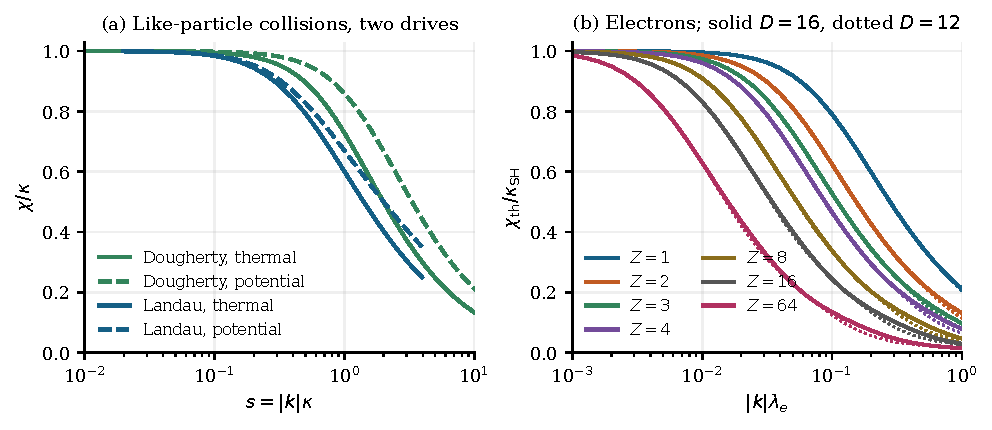
\includegraphics[width=\textwidth]{figures/responses.pdf}
\caption{(a) Like-particle operators at matched conductivity: the thermal
and potential drives share $\kap$ and differ beyond it. Dougherty curves
are the closed forms; Landau curves are Galerkin solves at $D=16$.
(b) Thermally driven electron response for several ion charges. The gap
between solid and dotted curves is the visible truncation error.}
\label{fig:responses}
\end{figure}

\subsection{Response curves and the two drives}

\Cref{fig:responses}(b) shows $\chi_\thr/\kap$ against $|k|\lambda_e$. At
$|k|\lambda_e=0.1$ the conductivity is $79\%$ of Spitzer--H\"arm for
$Z=1$ and $34\%$ for $Z=8$. The two degrees agree to plotting accuracy
for $|k|\lambda_e\lesssim0.1$ and separate beyond it, more so at large
$Z$. A polynomial basis cannot resolve the resonant layer at large
$|k|\lambda_e$, and we make no claim there. All curves lie between the
bounds \eqref{eq:bounds}.

\begin{table}[tb]
\centering
\caption{Like-particle Landau collisions: the conductivity and the
leading deficit coefficients for the potential and thermal drives.}
\label{tab:drives}
\small
\begin{tabular}{rrrrr}\toprule
$D$ & $\kappa/\tau$ & $K_{\rm pot}/\tau^2$ & $K_{\rm th}/\tau^2$ & ratio\\\midrule
6 & 3.906250 & 15.6779 & 19.5555 & 1.2473 \\
8 & 3.950050 & 22.4628 & 26.4761 & 1.1787 \\
10 & 3.950180 & 22.3786 & 26.3892 & 1.1792 \\
12 & 3.950196 & 22.3425 & 26.3532 & 1.1795 \\
16 & 3.950208 & 22.3477 & 26.3584 & 1.1795 \\
\bottomrule\end{tabular}

\end{table}

\Cref{fig:responses}(a) and \cref{tab:drives} compare the two drives for
like-particle collisions. For Landau the thermal coefficient is
$K_\thr/\tau^2\simeq26.36$, compared with $K_\pot/\tau^2\simeq22.35$, a
ratio of $1.18$. For Dougherty the ratio is $(16/45)/(2/15)=8/3$. In all
of our computations $\chi_\pot\geq\chi_\thr$; we have not proved this.
The thermally driven Landau response is positive and below $\kap$ at
every sampled $k$, which \cref{cor:bounds} now guarantees for the Galerkin
problem at any $k$ and, under \cref{ass:form}, for the continuum.

\subsection{An embedded test: decay of a temperature perturbation}\label{sec:embedded}

A static response has to be tested separately as an evolution law. The
natural experiment here is the decay of an electron temperature
perturbation, the setting of \cite{EpperleinShort1991}. The kinetic model
is \eqref{eq:kinetic} with $p=0$ and with the ambipolar force chosen at
each time so that the current vanishes:
\begin{equation}
 \partial_th=-P\,(ikv_x+\Lambda_Z)\,Ph,\qquad
 P=1-|v_x\rangle\langle v_x| ,\qquad h(0)=\tfrac12(|v|^2-3).
 \label{eq:kineticqn}
\end{equation}
The initial condition is a Maxwellian with a temperature perturbation,
$T(0)=1$ and $n=u=q=0$. The density and current remain zero, and
$\|h\|_{L^2(M)}$ is nonincreasing; we verify both numerically. The exact
energy equation is $\tfrac32\dot T=-ikq$, so the closed model is
\begin{equation}
 \tfrac32\dot T=-k^2\chi\,T .
 \label{eq:closed}
\end{equation}
We compare three choices of $\chi$: the quasi-static thermal response
$\chi_\thr(k)$, the local value $\kap$, and the value that makes
\eqref{eq:closed} decay at the rate of the least-damped kinetic mode
carrying temperature. Time is advanced with a matrix exponential, so
there is no time-step error. The error is the relative $L^2$ error of
$T(t)$ over six quasi-static decay times, computed with $601$ samples and
the trapezoidal rule. The reference uses $D=16$, and the column
``Refinement'' applies the same metric to the difference between the
$D=12$ and $D=16$ kinetic solutions.

\begin{table}[tb]
\centering
\caption{Embedded history error of the closed temperature equation
\eqref{eq:closed} for three conductivities. Errors smaller than the
refinement column are not resolved.}
\label{tab:embedded}
\small
\begin{tabular}{rrrrrrrr}\toprule
$Z$ & $|k|\lambda_e$ & $t_{\rm decay}/\tau_e$ & $\chi_{\rm th}/\kappa$ & Quasi-static & Spitzer--H\"arm & Least-damped & Refinement\\\midrule
1 & 0.01 & 4713 & 0.9957 & 0.0003 & 0.0031 & 0.0004 & 1.9e-03 \\
1 & 0.03 & 540.1 & 0.9654 & 0.0021 & 0.0248 & 0.0030 & 2.0e-03 \\
1 & 0.1 & 59.34 & 0.7907 & 0.0103 & 0.1561 & 0.0144 & 4.2e-03 \\
1 & 0.3 & 10.87 & 0.4798 & 0.0202 & 0.4230 & 0.0202 & 5.2e-04 \\
8 & 0.01 & 1818 & 0.9102 & 0.0015 & 0.0649 & 0.0020 & 8.9e-05 \\
8 & 0.03 & 274.8 & 0.6691 & 0.0038 & 0.2556 & 0.0051 & 2.9e-04 \\
8 & 0.1 & 49.01 & 0.3376 & 0.0401 & 0.5662 & 0.0693 & 6.7e-03 \\
8 & 0.3 & 12.4 & 0.1483 & 0.1141 & 0.7716 & 0.2220 & 5.3e-02 \\
\bottomrule\end{tabular}

\end{table}

\begin{figure}[tb]
\centering
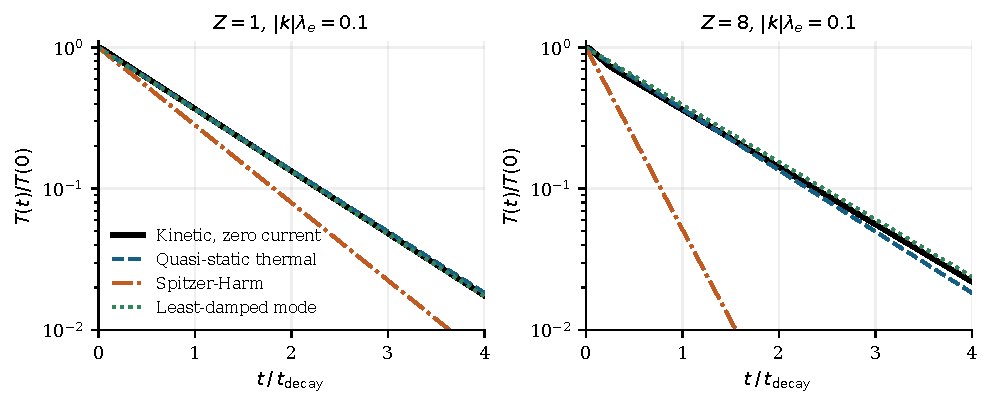
\includegraphics[width=\textwidth]{figures/embedded_decay.pdf}
\caption{Decay of a temperature perturbation at $|k|\lambda_e=0.1$ in
the quasi-neutral kinetic model and in the closed equation
\eqref{eq:closed}.}
\label{fig:embedded}
\end{figure}

\Cref{tab:embedded} and \cref{fig:embedded} give the results. For $Z=1$
the quasi-static closure has errors of $1\%$ at $|k|\lambda_e=0.1$ and
$2\%$ at $0.3$, where the conductivity has dropped to $48\%$ of its local
value and Spitzer--H\"arm conduction is off by $42\%$. For $Z=8$ the
errors are $0.4\%$ at $|k|\lambda_e=0.03$ and $4\%$ at $0.1$. The entry
at $Z=8$, $|k|\lambda_e=0.3$ has a refinement difference of $5\%$, so its
$11\%$ model error is only partly resolved, and we do not interpret it.
At the two smallest wavenumbers for $Z=1$ the model errors are below the
refinement difference, which there reflects the $0.3\%$ change in $\kap$
between degrees.

This is a much better outcome than the embedded test of the companion
manuscript, where the exact quasi-static closure had errors of $24\%$ and
$34\%$. We think the difference is the time scale. There, the temperature
was coupled to sound waves with frequencies comparable to the collision
rate. Here, quasi-neutrality removes the acoustic dynamics and the
temperature decays over $10$ to several thousand collision times
(\cref{tab:embedded}), so a zero-frequency response is the appropriate
one. It is interesting that the quasi-static closure is at least as
accurate as the least-damped-mode closure, which matches the late-time
rate exactly but not the initial layer.

\section{Discussion}\label{sec:discussion}

For closure benchmarks, the thermal drive is a better target than the
potential drive in three dimensions. It has a direct physical
interpretation for electrons, and its response satisfies
$0<\chi_\thr\leq\kap$ at every wavenumber for a large class of collision
operators. A learned symbol for the thermally driven flux can therefore
build in positivity and the Fourier upper bound without adding an
unjustified assumption, which is not the case for the potential drive.
The benchmark should record which drive generated its targets:
\cref{prop:matrix} shows that the two are different functions of one
response matrix, and they differ at order $k^2$.

The results also suggest how to hold out collision physics. The ion
charge is a one-parameter family along which the conductivity changes by
a factor of four and the normalized deficit by a factor of twenty. A
closure fitted at one value of $Z$ and matched to the local conductivity
at another will be wrong at order $k^2$ by a known amount.

Several steps toward realistic settings remain, and we list them in what
we think is increasing order of difficulty.
\begin{enumerate}
\item \emph{Certified constants and larger $|k|\lambda_e$.} A basis
adapted to the $|v|^{-3}$ singularity, or a speed grid, would remove the
slow convergence at large $Z$ and reach the collisionless layer.
\item \emph{A weighted existence theorem for $\Lambda_Z$.} The Lorentz
form adds coercivity in the angular directions, so we expect the weighted
argument of the companion manuscript to go through, but we have not
checked it.
\item \emph{Comparison with practical nonlocal models.} The constants
$\kap(Z)$ and $K(Z)$ are direct tests of the small-$k$ behavior of
multigroup diffusion and convolution closures
\cite{LMV1983,EpperleinShort1991,Brodrick2017}.
\item \emph{Frequency dependence.} The embedded test succeeds because the
dynamics are slow. Driven problems with frequencies comparable to the
collision rate need $\chi(k,\omega)$ or a retained heat flux.
\item \emph{Magnetization, ion dynamics, and nonlinear temperature
contrasts.} None of these is addressed here.
\end{enumerate}

\paragraph{Data and code availability.}
The directory containing this note holds the configuration, the numerical
module and its unit tests, the reproduction and plotting scripts, and the
saved metrics from which every table and figure is generated. The
like-particle Landau assembly is in
\texttt{shared/scripts/landau\_closure/}. No result depends on a training
run.

\FloatBarrier
\bibliographystyle{unsrtnat}
\bibliography{references}
\end{document}
